\chapter{Android}\label{cap:android}


\section{Introducción.}

Android es un sistema operativo basado en Linux, libre y multiplataforma. Inicialmente empezó como un sistema operativo solo para móviles pero con el tiempo ya podemos encontrarlo en móviles, tablets, pc, neveras, relojes, cámaras de fotos y una gran cantidad de aparatos.

En el proyecto lo usaremos para diseñar y desarrollar una aplicación móvil, con la que poder firmar digitálmente un texto leido previamente mediante un lector de códigos QR.

Android es propiedad de Google actualmente y es el encargado de dar soporte y ayudar a los desarrolladores. Esta función la realiza muy bien, dando una muy buena API y una gran documentación. Podemos encontrar toda la información que podemos necesitar para desarrollar una aplicación en la siguiente web, \url{http://developer.android.com/index.html}. En la anterior web podemos encontrar la documentación de la API, consejos de diseño para que la aplicación tenga un aspecto bonito a la vez que usable, todas las novedades incluidas en las versiones nuevas del sistema operativo, etc.

\section{Arquitectura de la plataforma Android.}

Como hemos dicho anteriormente Android es una plataforma que engloba desde el sistema operativo, al software intermedio que comunica el sistema operativo y las aplicaciones, llamado en inglés middleware y las posibilidad de hacer funcionar las aplicaciones en la plataforma elegida, ya sea un telefono, un tablet o cualquier aparato con Android.

Para los desarrolladores Android proporciona dos kit de desarrollo, uno que usa la tecnología Java (SDK), el que hemos usado en el proyecto y otro que da la posibilidad de programar a más bajo nivel (NDK), este último desarrollado en C++.

El SDK de Android proporciona ayuda para las siguientes características, un navegador basado en WebKit, graficos optimizados en 2D, gráficos en 3D basados en OpenGL ES 1.0 con aceleración gráfica, una base de datos para almacenar datos que necesitemos, llamada SQLite, soporte para ficheros gráficos (JPG, PNG, GIF, etc), vídeo (MPEG4, H.264) y audio (MP3, AAC), telefonía GSM, tecnologías inalámbricas como son Bluetooth, 3G, Wifi, uso de la cámara, GPS, brújulas, etc. Además de todo esto, proporciona ayuda en la reutilización y remplazo de componentes, una máquina virtual optimizada para dispositivos móviles llamada Dalvik y un emulador donde poder probar la aplicación antes del lanzamiento sin tener que poseer un terminal Android. 

\begin{figure}
  \centering
    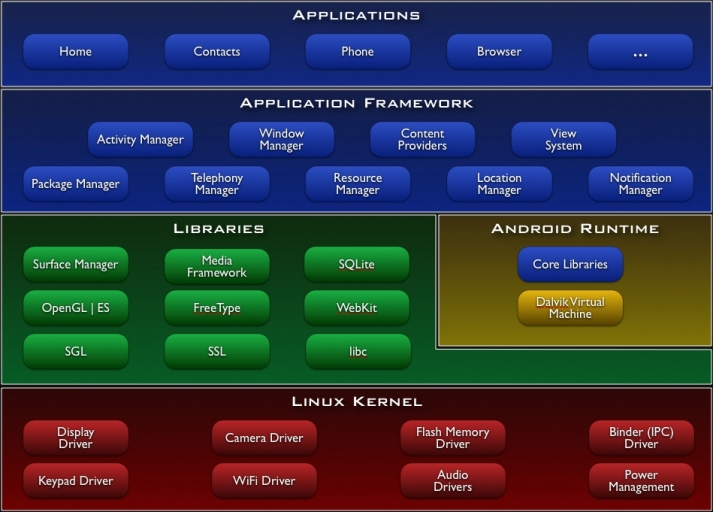
\includegraphics[scale=0.6]{./Android/imagenes/arquitecturaAndroid.jpg}
  \caption{Arquitectura de Android.}
  \label{fig:arquitecturaAndroid}
\end{figure} 

La arquitectura la podemos ver en la figura~\ref{fig:arquitecturaAndroid}. En la imagen podemos observar las cinco capas principales en las que se divide Android.
\begin{itemize}

\item \textbf{Applications:} en esta capa están todas las aplicaciones que nos proporciona el sistema operativo de base, como pueden ser la lista de contactos, un gestor de SMS, el navegador, el lanzador de aplicaciones, todas las aplicaciones de servicios de Google, como pueden ser Gmail, Google Maps, Google Calendar, Google Reader.   

\item \textbf{Application framework:} en esta capa está todo lo relacionado con los manejadores de activitys, llamadas de telefono, controladores de vistas. Es una capa que hay intermedia para manejo de hardware, con la que se pueden controlar tanto las notificaciones, como servicios que se ejucutan en segundo plano, etc. Los desarrolladores tienen el mismo acceso mediante esta capa de la API a todos los servicios que las aplicaciones nativas que proporciona el sistema el operativo. 

\item \textbf{Libraries:} como su nombre indica en esta capa están todas las librerías que el sistema operativo necesita, para manejo de archivos multimedia, manejo de gráficos 3D, renderizado web, etc.

\begin{itemize}
	\item \textbf{System C library:} una implementación del estandar C, optimizada para funcionar en sistemas móviles para las funciones del kernell de linux.
	\item \textbf{Media Libraries:} librerías basadas en PacketVideo's OpenCORE para grabación y reproducción de formatos de audio y video mas populares del momento como MP3, H.264, JPG o PNG.

	\item \textbf{Surface Manager:} librería para manejo de graficos 2D y 3D para varias aplicaciones.

	\item \textbf{LibWebCore:} motor de renderizado para navegadores embebidos de páginas web.

	\item \textbf{SGL:} motor para renderizado 2D.

	\item \textbf{3D libraries:} librería que implementa la API de OpenGL ES 1.0, que proporciona aceleración 3D por hardware si es posible o una alta optimización para renderizado por software en sistemas que no posean aceleración por hardware.

	\item \textbf{FreeType:} librería para manejo de fuentes, tanto bitmap como vectoriales.

	\item \textbf{SQLite:} librería para el manejo de la base de datos que proporciona Android.

\end{itemize}

%si hablo de la máquina virtual algo más poner una referencia.
\item \textbf{Android Runtime:} es una capa que está al mismo nivel que la capa de librerías. En esta capa se añaden muchas librerías para dotar de la mayoría de las funcionalidades que proporciona Java, también está en esta capa la máquina virtual (Dalvik) encargada de ejecutar el código Smali de los archivos DEX.

\item \textbf{Linux Kernel:} Android está basado en el kernel de Linux 2.6 y todo lo relatico a seguridad, manejo de memoria, control de procesos, pila de protocolos de red y modelo de drivers es el mismo. El kernel es el que proporciona una capa de abstracción entre el hardware y el software que usará Android.

\end{itemize}

Como ya hemos dicho antes Android corre cada aplicación en una máquina virtual, esta máquina virtual recibe el nombre de Dalvik. Dicho nombre viene de un pueblo de Islandía donde viven los familiares del creador de esta, Dan Bornstein. La máquina virtual ejecuta un byte code especial llamdo DEX (Dalvik Executable), que está especialmente diseñado y optimizado para funcionar en sistemas móviles, tablets, etc. En la figura~\ref{fig:maquinaVirtualDalvik} podemos ver todo el proceso desde la creación del archivo JAVA a la ejecución.

\begin{figure}[h]
  \centering
    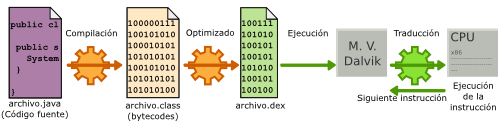
\includegraphics[scale=0.8]{./Android/imagenes/maquinaVirtualDalvik.png}
  \caption{Proceso de ejecución en Android.}
  \label{fig:maquinaVirtualDalvik}
\end{figure}


Los ficheros DEX meten las cadenas duplicadas y las constantes en un mismo fichero para ahorrar espacio, normalmente los archivos DEX suelen ser más pequeños que los archivos JAR de la máquina virtual Java. Una vez instados los archivos DEX pueden ser modificados en el terminal para añadir optimizaciones, reordenado de byte en ciertos datos, quitado de clases vacias, etc. En la versión 2.2 de Android se añadió una nueva característica llamada JIT (Just-In-Time) que es compilación en tiempo real de los archivos DEX, por lo que se pueden añadir nuevas optimizaciones dependiendo de la plataforma.

Todas las aplicaciones de Android se distribuyen en unos archivos con extensión APK. Estos archivos no son más que archivos ZIP con la extensión cambiada. Todos deben tener una estructura idéntica, que se explica a continuación. Contiene diferentes carpetas en las que se incluyen ficheros de configuración, fiecheros necesarios para el funcionamiento de la aplicación y para comprobar la integridad de los mismos.

\begin{itemize}

\item \textbf{META-INF:} en un directorio que contiene tres archivos, \textit{MANIFEST.MF} que es el archivo de manifest, \textit{CERT.RSA} que es el certificado con el que está firmada la aplicación, \textit{CERT.SF} que contiene el hash en SHA-1 de todos los componentes de la aplicación, un ejemplo del archivo \textit{CERT.SF} es el siguiente:

\begin{verbatim}

Signature-Version: 1.0
Created-By: 1.0 (Android)
SHA1-Digest-Manifest: wxqnEAI0UA5nO5QJ8CGMwjkGGWE=
...
Name: res/layout/exchange_component_back_bottom.xml
SHA1-Digest: eACjMjESj7Zkf0cBFTZ0nqWrt7w=
...
Name: res/drawable-hdpi/icon.png
SHA1-Digest: DGEqylP8W0n0iV/ZzBx3MW0WGCA=
\end{verbatim}

\item \textbf{lib:} esta carpeta puede contener otras dependiendo de la plataforma para la que esté diseñada la aplicación. Si por ejemplo tiene código específicamente diseñado para x86 tendrá una carpeta llamada x86, si tiene código para MIPS una llamada mips donde se encontraría el código especialmente diseñado para esta plataforma. Puede que dicha carpeta no exista.

\item \textbf{res:} este directorio contiene todos los recursos que no tienen que ser compilados, como pueden ser imágenes, sonidos, etc.

\end{itemize}

Además de estas carpetas todos los ficheros APK incluyen estos tres archivos.

\begin{itemize}
\item \textbf{AndroidManifest.xml:} es un archivo que sirve para indicar la versión, los permisos que contiene la aplicación, las referencias a librerías, las activitys que contiene la aplicación. En el siguiente listado podemos observar un extracto de los permisos que usamos en la aplicación del proyecto.

\begin{lstlisting}[style=XML]
<uses-permission android:name="android.permission.INTERNET" />
<uses-permission android:name="android.permission.WRITE_EXTERNAL_STORAGE" />
<uses-permission android:name="android.permission.WRITE_SETTINGS" />
<uses-permission android:name="android.permission.GET_ACCOUNTS" />
<uses-permission android:name="android.permission.USE_CREDENTIALS" />
<uses-permission android:name="android.permission.MANAGE_ACCOUNTS" />
\end{lstlisting}

Podemos ver que con esto garantizamos que la aplicación pueda conectarse a internet, usar la tarjeta SD y manejar las cuentas almacenadas en el móvil, como puede ser la dirección de correo usada para dar de alta el móvil en Google Play.

\item \textbf{classes.dex:} el archivo DEX donde están todas las clases precompiladas en byte code para la máquina virtual Dalvik.

\item \textbf{resources.arsc:} es un fichero que contiene los recurdos precompiados como pueden ser los XML de las interfaces de la aplicación, etc.

\end{itemize}

En la imagen~\ref{fig:estructuraAPK} se pueden observar los ficheros y las carpetas comentadas anteriormente del proyecto.

\begin{figure}[h]
  \centering
    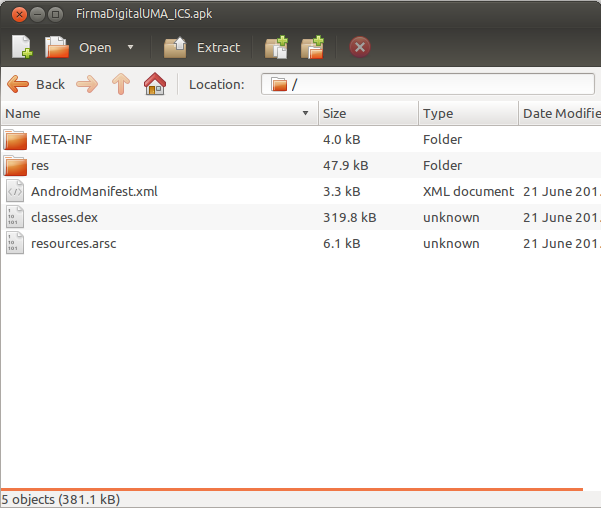
\includegraphics[scale=0.8]{./Android/imagenes/estructuraAPK.png}
  \caption{Estructura del fichero APK del proyecto.}
  \label{fig:estructuraAPK}
\end{figure}

Toda aplicación en Android se contruye con unos componentes básicos como pueden ser activities, intents, views, services, contents providers, widgets y un largo etcétera. A continuación vamos a explicar los más importantes.

\begin{itemize}

%poner sección
\item \textbf{Activity:} una activity es la entidad más básica de una interfaz de usuario donde se puede mostrar información en Android, podemos pensar que es como una ventana de cualquier aplicación de escritorio. Cada interfaz que vemos en una aplicación de Android es una activity. Android tiene un ciclo de manejo de activitys bastante complejo, se explicará en la sección~\ref{cap:desarrolandoAndroid} donde pondremos más incapié en el desarrollo de la aplicación móvil del proyecto.

\item \textbf{Intent:} un intent es un componente practicamente imprescindible en cualquier aplicación de Android, es una forma de comunicación entre cualquier componente. Se pueden definir como mensajes o peticiones, ya que también puede comunicar aplicaciones entre sí. En el proyecto usamos intent para comunicar las activities y poder intercambiar datos entre ellas, también la usamos para abrir el lector de códigos QR que necesitamos, dentro de nuestra aplicación llamamos al intent que nos proporciona la aplicación lectora y cuando termine ella nos devuelve el valor que había en el código QR para que podamos tratarlo.

\item \textbf{View:} son los componentes básicos con los que podemos contruir las interfaces gráficas, como pueden ser botones, barras de texto, campos de texto, spinner, etc. Android pone a nuestra disposición una gran cantidad de estos elementos, y además brinda la posibilidad de crear nuevos, según los vayamos necesitando. Estos objetos normalmente se añaden a una vista y se pueden añadir, modificar o borrar en ella. Estos objetos tienen un ID único en la aplicación por el que podemos controlarlo y añadirle por ejemplo el texto si es un campo de texto o un listener si es un botón para que cuando se pulse realizar la acción que necesitemos.

\item \textbf{Services:} un servicio es un componente de Android que no tiene interfaz gráfica asociada y se ejecuta en segundo plano. Es similar a los servicios que ofrece cualquier sistema operativo. Pueden realizar cualquier acción, tanto recoger o actualizar datos, lanzar notificaciones cada cierto tiempo o mostrar activity para que el usuario introduzca algún valor que necesite.

\item \textbf{Content Provider:} es un mecanismo que posee Android para intercambiar información entre aplicaciones. Por ejemplo cuando usamos la opción de compartir en el teléfono, dentro de una aplicación, nos salen varias aplicaciones con las que podemos compartir directamente, estas son todas las aplicaciones que han implementado el content provider que necesita esta aplicación para compartir la información. En la figura~\ref{fig:contentProvider} podemos ver la opción de compartir de una aplicación y podemos observar como aparece por ejemplo GMail para mandar un email directamente desde aquí sin tener conocimiento de como se produce el intercambio de datos.
 
\begin{figure}[h]
  \centering
    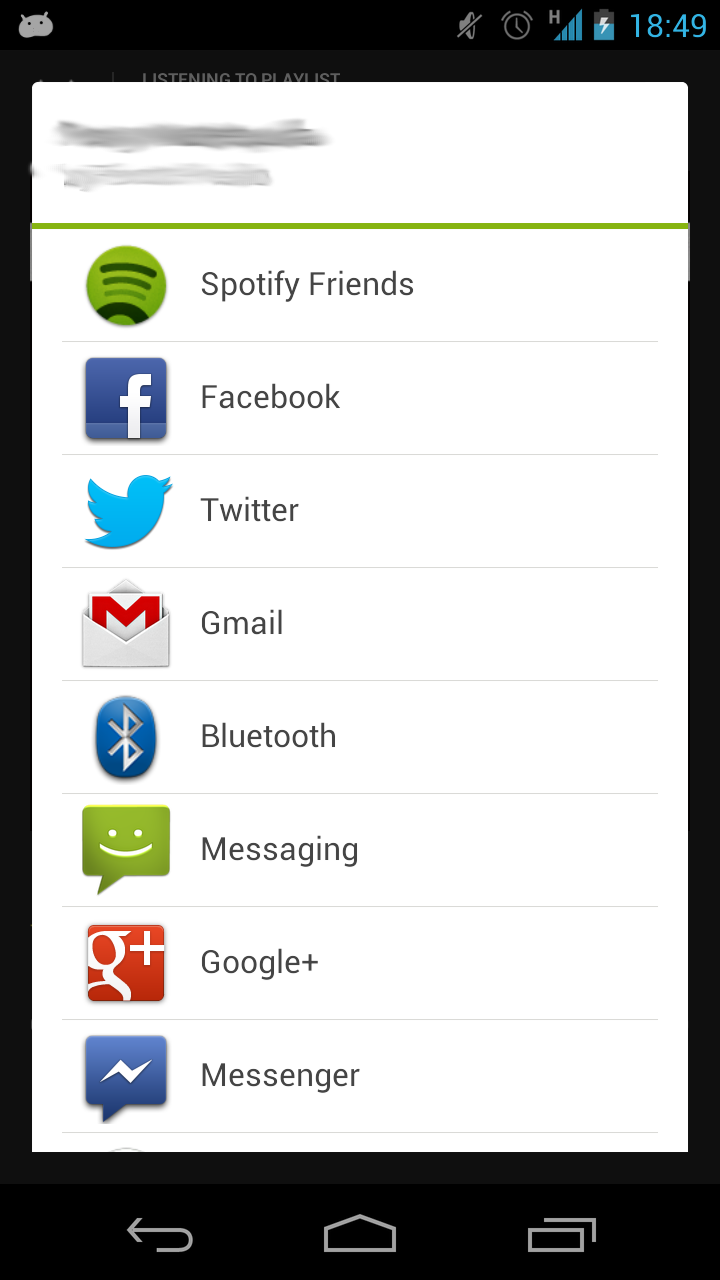
\includegraphics[scale=0.2]{./Android/imagenes/contentProvider.png}
  \caption{Opción compartir de una aplicación.}
  \label{fig:contentProvider}
\end{figure}

\item \textbf{Broadcast Receiver:} es un componente de Android diseñado para actuar cuando ocurre un evento general del sistema, como puede ser la recepción de un SMS, la batería se está agotando, una llamada entrante, etc. También una aplicación puede generar eventos de este tipo para que cualquiera que implemente un Broadcast Receiver pueda recibirlo.

\item \textbf{Widget:} son elementos visuales y generalmente para que el usuario realice alguna acción, tales como poner en pausa la música, pasar de canción, revisar los feed RSS, mirar los correos pendientes, etc. Suele estar en alguna de las pantallas principales de Android. En la figura~\ref{fig:widget} podemos ver un widget de GMail.
 
\begin{figure}[h]
  \centering
    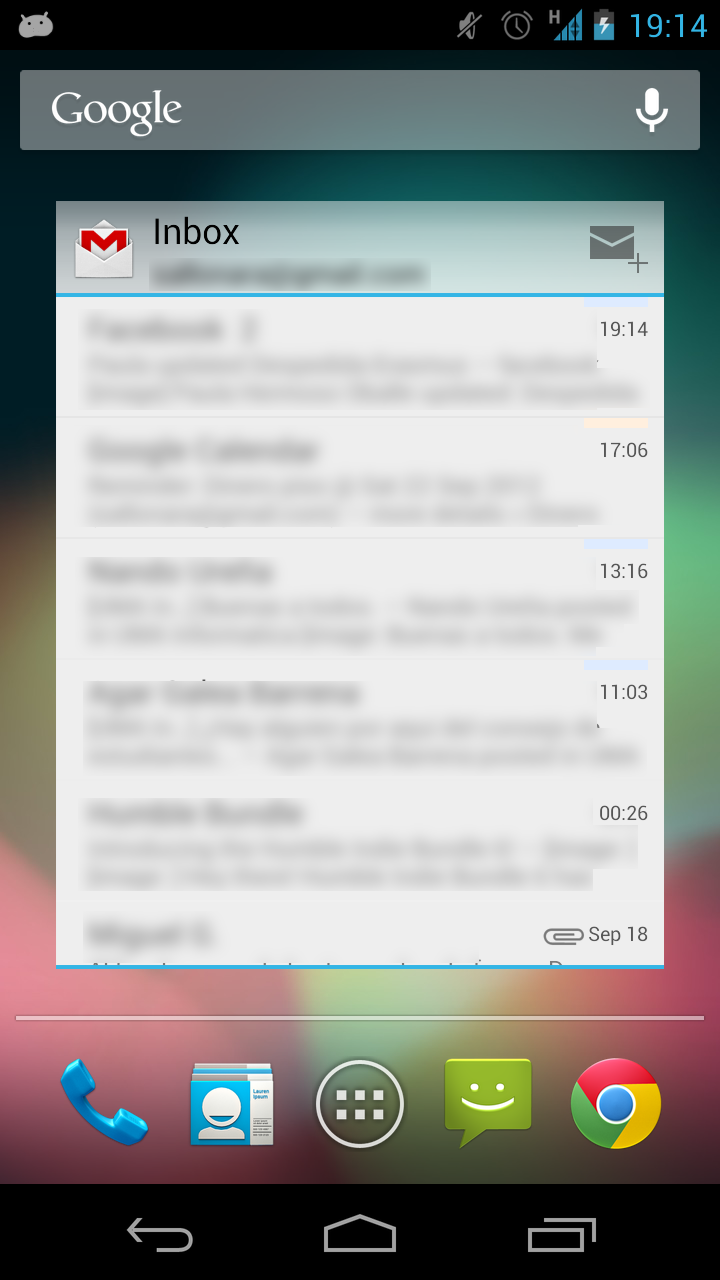
\includegraphics[scale=0.2]{./Android/imagenes/widget.png}
  \caption{Widget de GMail.}
  \label{fig:widget}
\end{figure}

\subsection{Desarrollando en Android.}\label{cap:desarrolandoAndroid}

Como ya hemos dicho anteriormente para el desarrollo de la aplicación móvil hemos usado el IDE de programación Eclipse. En el anexo~\ref{cap:apendiceA} podemos ver como realizar la configuración de Eclipse para la programación de aplicaciones Android. En la sección~\ref{cap:proyectoBasico} se explicará con más detenimiento la estructura de un proyecto básico en Android.

En este apartado vamos a explicar las entidades más importantes que existen en Android, como pueden ser las activity, fragment, y view usados en el proyecto.

En el proyecto la entidad más importante que hemos usado es la \lstinline{Activity}. Normalmente las activity están enfocadas a interactuar con el usuario de alguna forma, ya puede ser necesitando de alguna acción del usuario o mostrando información y normalmente ocupan toda la pantalla del terminal, pero puede flotar dentro de otra activity o agruparse con otras usando la clase \lstinline{ActivityGroup}. Todas las subclases que hereden de \lstinline{Activity} tienen que implementar dos métodos impresindibles. Estos son \lstinline{onCreate(Bundle)} y \lstinline{onPause()}. El primero es donde se inicializa la activity y en el segundo es lo que ocurre cuando el usuario abandona la activity.

Habitualmente toda Activity tiene asociada una interfáz gráfica que se diseña en un fichero XML, como veremos posteriormente, este archivo se le indica a cada Activity con el método \lstinline{setContentView(int);} al cual hay que pasarle una constante que genera automáticamente la clase \lstinline{R} de Android. Una vez se le ha indicado el archivo XML se puede obtener cada uno de los componentes (botones, cuadros de texto, etc) que componen la intefaz gráfica con el método \lstinline{findViewById(int)}. Todo este proceso se tiene que realizar dentro del método \lstinline{onCreate();} y se puede observar en el siguiente trozo de código.

\begin{lstlisting}[style=Java]
@Override
protected void onCreate(Bundle savedInstanceState) {
	super.onCreate(savedInstanceState);
	setContentView(R.layout.initialconfigurescreen);

	TextView tAccountOk = (TextView) findViewById(R.id.tAccountOk);
	EditText tCertificate = (EditText) findViewById(R.id.tCertificate);
	ImageView image = (ImageView) findViewById(R.id.imageView1);

	Button bSelectAccount = (Button) findViewById(R.id.bConfigureScreenAccount);
}
\end{lstlisting}

A continuación vamos a explicar las características y su ciclo de vida de las Activity, ya que es un tema muy importante cuando desarrollamos una aplicación Android. En la figura~\ref{fig:cicloActivity} podemos ver todos los estados por los que pasa una Activity desde que se crea hasta que finaliza. 

\begin{figure}
  \centering
    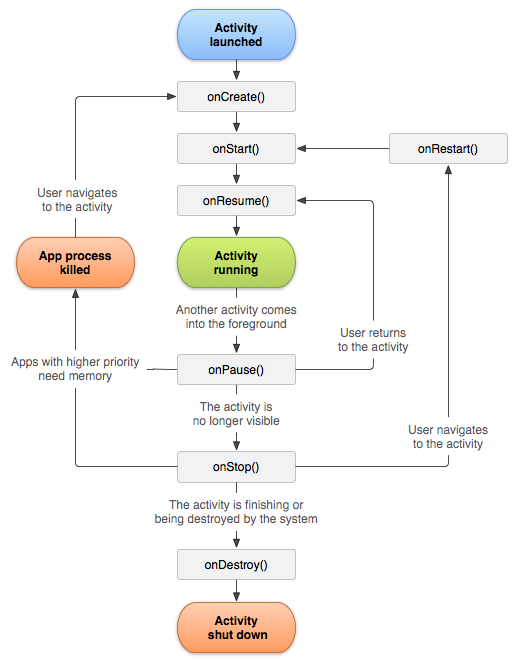
\includegraphics[scale=0.8]{./Android/imagenes/cicloActivity.png}
  \caption{Ciclo de vida de una activity.}
  \label{fig:cicloActivity}
\end{figure}

Todos estos estados se pueden controlar mediante la implementación en la clase que hereda de \lstinline{Activity} de los siguientes métodos.

\begin{lstlisting}[style=Java]
public class Activity extends ApplicationContext {
	protected void onCreate(Bundle savedInstanceState);

	protected void onStart();

	protected void onRestart();

	protected void onResume();

	protected void onPause();

	protected void onStop();

	protected void onDestroy();
}
\end{lstlisting}

Como podemos ver en la figura \ref{fig:cicloActivity} podemos ver que el ciclo completo de una activity es desde el método \lstinline{onCreate(Bundle);} hasta que se realiza la llamada al método \lstinline{onDestroy();}. Como hemos visto antes en \lstinline{onCreate(Bundle);} se genera todo lo necesario para que la activity funcione, como puede ser la inicialización de la interfaz, la creación de un hilo para que realice una operación en background o cualquier otra acción que necesite ser inicializada. El método \lstinline{onDestroy();} se pararía el hilo y se liberá la memoria usada por la activity. Entre los procesos \lstinline{onStart();} y \lstinline{onStop();} es donde se mantienen los recursos para que la activity pueda mostrar los datos al usuario. Por ejemplo si tenemos un \lstinline{BroadcastReceiver}, que nos puede cambiar la interfaz de usuario pues lo registramos en el método \lstinline{onStart();} y lo paramos en \lstinline{onStop();}. Estos dos métodos se llaman mucho a lo largo de la ejecución de la activity cada vez que el usuario oculta la activity y vuelve a ejecutarla. Los métodos \lstinline{onResume();} y \lstinline{onPause();} se usan para intercambio de activity, cuando apagamos la pantalla del móvil y volvemos a encenderla, cuando giramos la pantalla, etc. En estos métodos se suelen usar \lstinline{Bundle} para intercambiar información entre los estados y así conseguir por ejemplo restaurar el texto de un cuadros de texto cuando vuelve a generarse.

En esta tabla podemos observar en cada estado del ciclo de vida de una activity puede ser matada y cual sería el próximo estado.
\begin{center}
\begin{tabular}{|l | c | r|}

\hline
Method & ¿Terminable? & Proximo estado\\
\hline
onCreate() & No & onStart()\\
\hline
onRestart() & No & onStart()\\
\hline
onStart() & No & onResume() o onStop()\\
\hline
onResume() & No & onPause()\\
\hline
onPause() & No  & onResume() o onStop()\\
\hline
onStop() & Sí & onRestart() o onDestroy()\\
\hline
onDestroy() & Sí & Ninguna\\
\hline

\end{tabular}
\end{center}
Antes de la versión 3.0 de Android las activity tenian que ocupar toda la ventana y para cambiar o mostrar otra pantalla había que generar una nueva activity de la siguiente forma:

\begin{lstlisting}[style=Java]
Intent intent = new Intent(activity, SplashScreenActivity.class);
startActivity(intent);
\end{lstlisting}

Ese trozo de código se ejecuta en una activity y podemos ver que se crea un objetos \lstinline{Intent} al cual se le dice la activity en la que está y la activity que tiene que iniciar, en este caso la variable \lstinline{activity} es la actual, y \lstinline{SplashScreenActivity} es una activity que tiene la función de inciar todas las variables y realizar las conexiones básicas en el proyecto, acto seguido se usa el procedimiento \lstinline{startActivity(intent);} al que se le pasa el objeto \lstinline{Intent} creado anteriormente y con esto tendríamos la nueva activity ejecutándose.

Desde la versión 3.0 y posteriores las activity siguen ocupando toda la pantalla pero se dio la posibilidad al programador de que usara solo trozos de ella con una clase llamada \lstinline{Fragment} de esta forma no tendría que iniciar una nueva activity cada vez que quiera modificar la interfáz, de este modo se pudieron empezar a usar gestos de scroll laterar para mostrar varias interfaces o en pantallas grandes como una tablet poder modificarla sin tener que generar una nueva activity. 
\begin{figure}
  \centering
    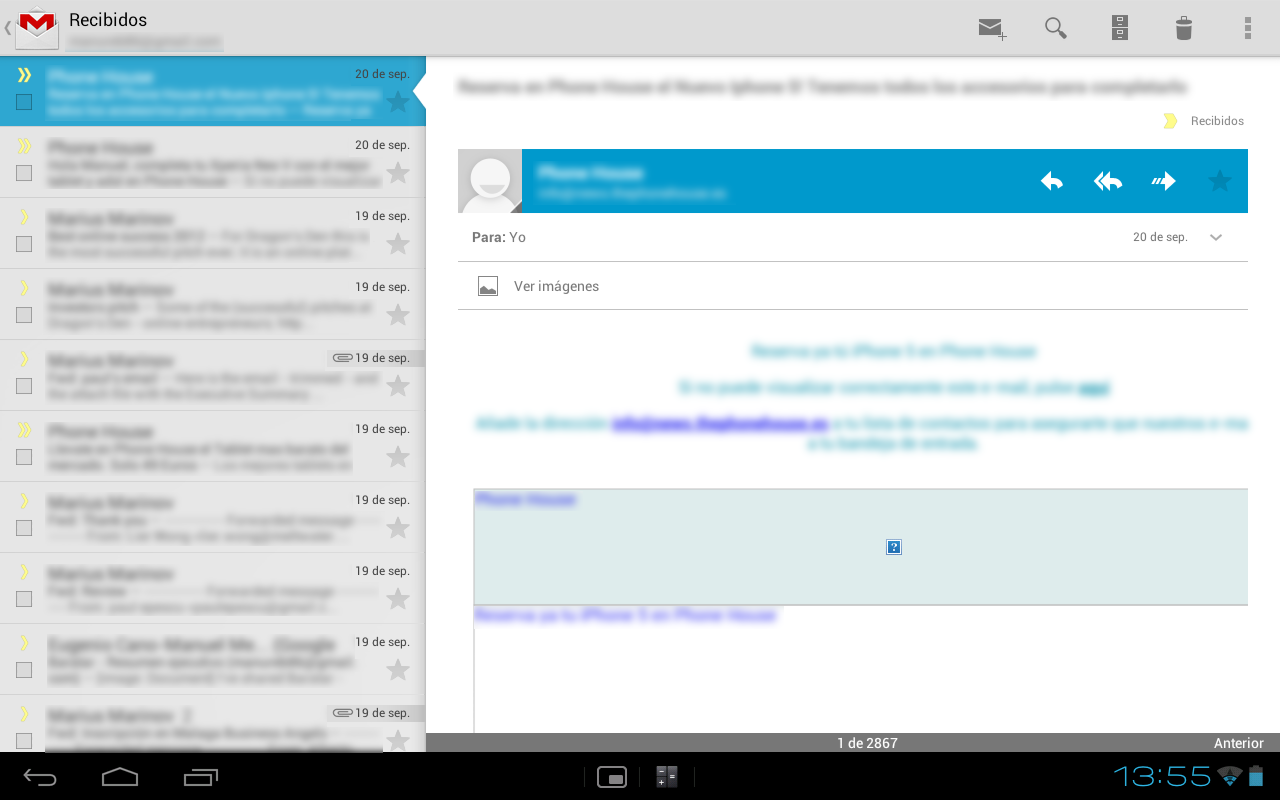
\includegraphics[scale=0.3]{./Android/imagenes/gmailTablet.png}
  \caption{Aplicación de Gmail para tablet.}
  \label{fig:gmailTablet}
\end{figure}

\begin{figure}
  \centering
    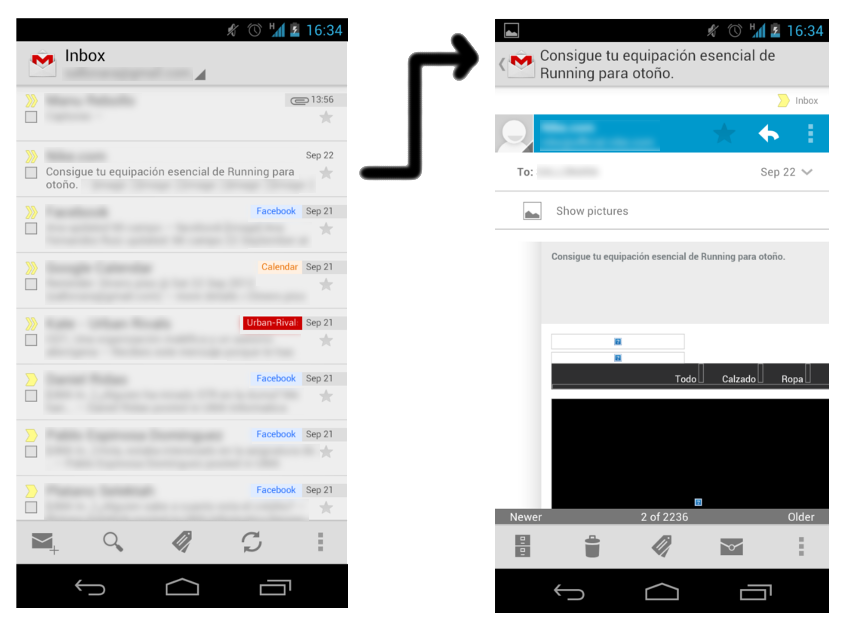
\includegraphics[scale=0.4]{./Android/imagenes/gmailMovil.png}
  \caption{Aplicación de Gmail para móvil.}
  \label{fig:gmailMovil}
\end{figure}

\begin{figure}[h]
  \centering
    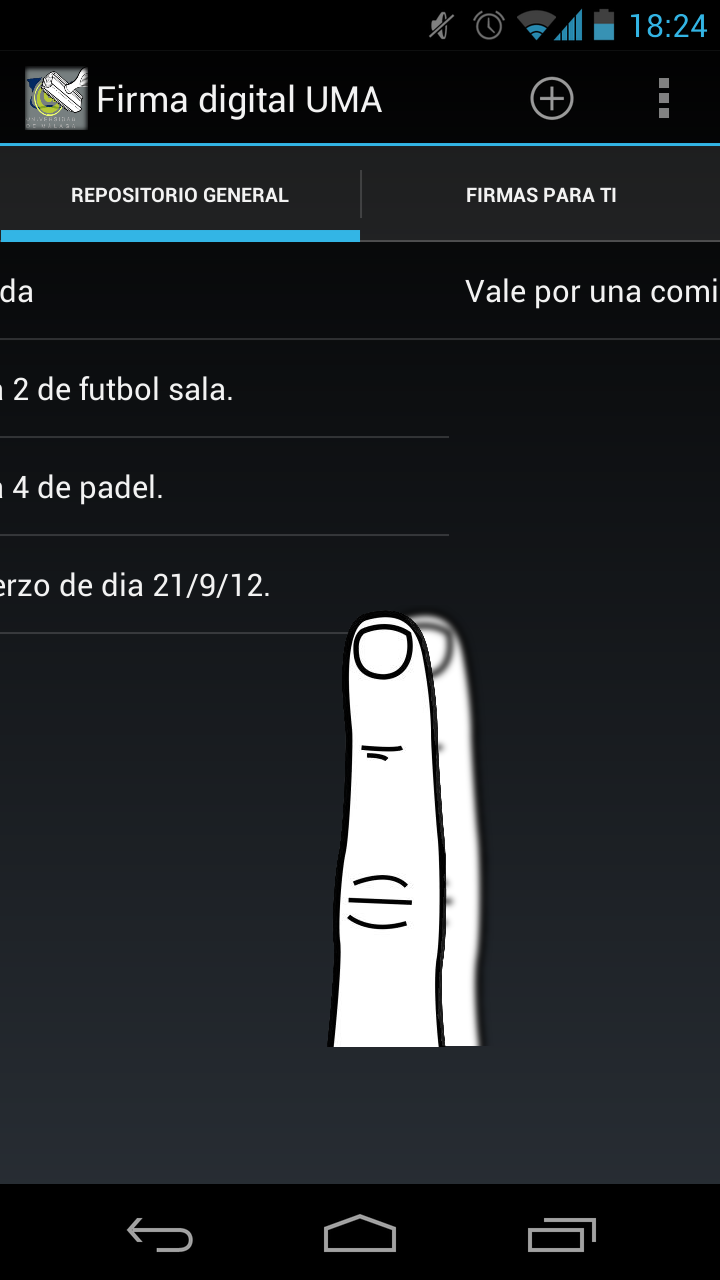
\includegraphics[scale=0.2]{./Android/imagenes/swype.png}
  \caption{Gesto Swype en la aplicación móvil.}
  \label{fig:swype}
\end{figure}

En la imagen~\ref{fig:gmailTablet} podemos ver la aplicación de Gmail diseñada mediante fragment y en ella si pulsamos algún correo en la parte izquierda de la aplicación nos mostraría el correo en la derecha sin tener que recagar la aplicación. En la imagen~\ref{fig:gmailMovil} podemos ver como en la versión movil no se usa esta forma por falta de espacio en la pantalla. Nosotros hemos realizado un diseño para intercambio de fragment mediante un gesto llamado swype o scroll lateral y como se puede ver en la imagen~\ref{fig:swype} podemos ver que no hay que volver a cargar otra activity ni nada, por lo que dotamos a la aplicación de una mayor fluidés.

Para que una aplicación pueda usar una determinada activity, el programador primeramente tiene que definir el uso y su función en el archivo \textit{AndroidManifest.xml}. Podemos ver un extracto de dicho archivo donde definimos un par de activity usadas en el proyecto.

\begin{lstlisting}[style=XML]
<activity android:name=".FirmaDigitalUMA_ICSActivity" />
<activity android:name=".InitialConfiguration" android:noHistory="true" />
\end{lstlisting}

Se puede observar que hemos declarado dos activities una sin ninguna opción y otra en la que no se guardará en la pila de llamadas de activity, por lo que si pulsamos el botón atrás no se abrirá de nuevo. Si no realizamos este proceso nos dará un error en tiempo de ejución la aplicación diciendo que hemos intentado ejecutar una activity que no está declarada.

\subsection{Proyecto básico de Android en Eclipse.}\label{cap:proyectoBasico}

A continuación vamos explicar con más detenimiento la estructura que tiene un proyecto básico de Android en Eclipse.

\begin{figure}
  \centering
    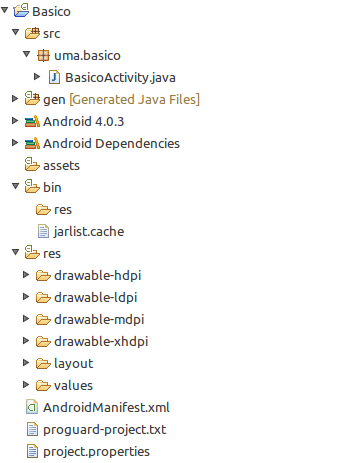
\includegraphics[scale=1]{./Android/imagenes/estructuraBasicaAndroid.png}
  \caption{Estructura básica de un proyecto Android.}
  \label{fig:estructuraBasicaAndroid}
\end{figure}

En la figura~\ref{fig:estructuraBasicaAndroid} podemos ver una captura de un proyecto recien creado. Podemos observar que se genera una carpeta principal en la que posteriormente colgarán el resto de carpetas necesarias. Estas carpetas son \textit{src}, \textit{gen}, \textit{assets}, \textit{bin}, \textit{res} y varios archivos sueltos como con \textit{AndroidManifest.xml}, \textit{proguard-project.txt}, \textit{project.properties}, vamos a explicar brevemente que contiene y cual es la función de dichas carpetas y documentos.

\begin{itemize}

\item \textbf{src:} en esta carpeta están todos los paquetes que contiene los archivos de código fuente que se necesitan en el proyecto.

\item \textbf{gen:} esta carpeta es donde se almacena todo lo que el proyecto de Android necesita para funcionar, casi todos los ficheros que se encuentran en el interior se generan cada vez que se construye el proyecto y si los modificamos nosotros, cuando volvamos a construir el proyecto borrarán los cambios. Dentro está la clase \lstinline{R} donde se declaran la mayoría de las constantes con direcciones de memoria que luego en tiempo de ejecución se usarán para realizar la conversión en bytecode del archivo java.

\item \textbf{bin:} es una carpeta donde se almacenan todos los archivos binarios, como puede ser el archivo APK, los archivos DEX, etc.

\item \textbf{res:} esta carpeta la encargada de contener todos los recursos necesarios para nuestra aplicación. Esta carpeta se divide en varias, como por ejemplo \textit{drawable-hdpi}, \textit{drawable-ldpi}, \textit{drawable-mdpi}, \textit{drawable-xhdpi} es donde se añaden todas imágenes usadas, sonidos, videos, etc. Pero no todos los recursos son contenido multimedia, hay otras carpetas como por ejemplo la carpeta \textit{layout} donde se almacenan las diferentes interfaces usadas en el en formato XML o la carpeta \textit{values} donde se guardan todas las cadenas constantes en un archivo XML.

\item \textbf{AndroidManifest.xml:} como ya hemos explicado anteriormente es el archivo donde se declara todos los permisos e información de interes de la aplicación, como pueden ser las activity, los intent, la versión mínima que tiene que tener el móvil para ejecutar nuestra aplicación, etc.  

\item \textbf{project.properties:} es un archivo donde se pueden configurar diferentes parámetros del proyecto, como puede ser la API sobre la que se va a ejecutar el proyecto, o si queremos usar una herramienta que ofrece Google dentro del SDK para ofuscar el código llamada ProGuard.

\item \textbf{proguard-project.txt:} ProGuard como hemos dicho antes es una herramienta que ofrece Google dentro del SDK de Android para ofuscación de código, ya que hay muchas herramientas de ingeniería inversa que mediante la decompilación de los archivos DEX se puede llegar casi a conseguir el código realizado sin permiso. En este archivo se puede configurar los diferentes valores para el uso de esta herramienta, tales como son que tipo de ofuscación queremos utilizar si solo sintáctica o semántica, si queremos que se pueda tracear la salida del archivo, etc. Para amplicar conocimientos sobre dicha herramienta podemos visitar esta web, \url{http://developer.android.com/tools/help/proguard.html} donde está toda la información necesaria.

\end{itemize}

%%---------------------------------------------
%%Cortar por aquí para pegar en implementación
%%---------------------------------------------

\section{Proyecto Firma Digital UMA.}

La aplicación Firma Digital UMA es la aplicación móvil que hemos realizado para facilitar la firma y visualización de nuevos documentos. En ella  podemos firmar nuevos documentos o comprobar los anteriormente firmados de una forma fácil, el resto de gestiones se pueden realizar desde la aplicación web, donde se puede verificar, generar nuevos documentos para que sean firmados, etc. En la figura~\ref{fig:pantallaPrincipal} podemos ver el aspecto de la aplicación.

\begin{figure}[h]
  \centering
    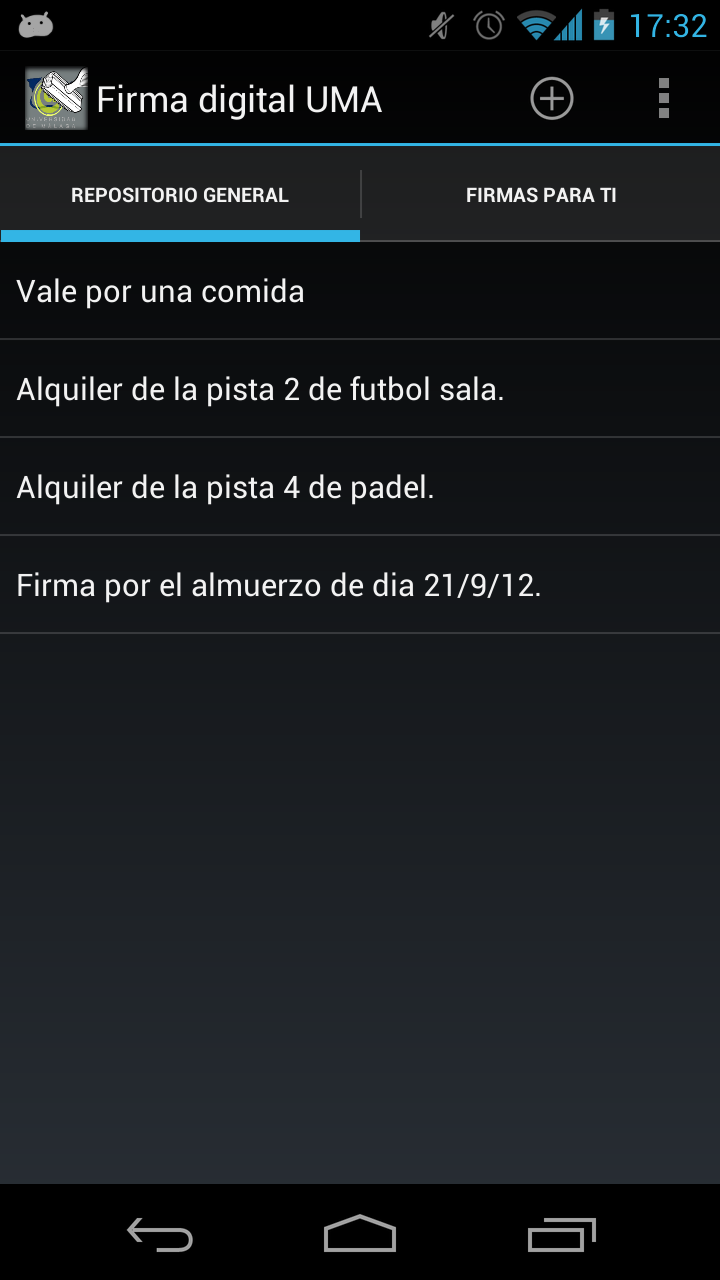
\includegraphics[scale=0.2]{./Android/imagenes/pantallaPrincipal.png}
  \caption{Pantalla inicial de la aplicación.}
  \label{fig:pantallaPrincipal}
\end{figure}

\subsection{Uso de la aplicación.}

Lo primero que pensamos cuando nos pusimos a diseñar la aplicación era que el método de firma tenía que ser rápido y fácil de realizar, por lo que se decidió usar los códigos QR para agilizar la lectura de información. Solo hay que pulsar el botón de añadir nuevo recibo (figura~\ref{fig:botonAnhadir}) y se abrirá el lector de códigos QR, una vez leidos el código este se firmará y se subirá automaticamente al servidor sin necesidad de que el usuario realice otra acción.

\begin{figure}[h]
  \centering
    
\includegraphics[scale=0.2]{./Android/imagenes/botonAnhadir.png}
  \caption{Detalle del botón añadir.}
  \label{fig:botonAnhadir}
\end{figure}

La aplicación se puede dividir principalmente en dos partes claramente diferenciadas, una en la que se muestra las firmas realizadas y otra en la que se muestran que tienen como destino el usuario que está ejecutando la aplicación. Las dos partes son practicamente idénticas y tienen el mismo uso. Si pulsamos encima de cualquier recibo de la lista nos mostrará toda la información de dicha firma, podemos ver un ejemplo en la figura~\ref{fig:informacionFirma}. Podemos observar todos los datos necesarios, como pueden ser destino, quien ha realizado la firma, la fecha, el texto, etc y también podemos ver si está verificada con el tick de color verde o una señal de error roja en caso contrario, que podemos ver en la esquina superior derecha. En el caso de los recibos de los que se es destino se indica de una forma más clara quien es el que usuario que envia el mensaje, pero el resto de la información es la misma.

En la información que nos proporcionan podemos ver la dirección del servidor de tiempo usado y si pulsamos en ella se abrirá el navegador con una dirección donde podremos confirmar el hash y la fecha en la que se realizó la firma.

\begin{figure}
  \centering
    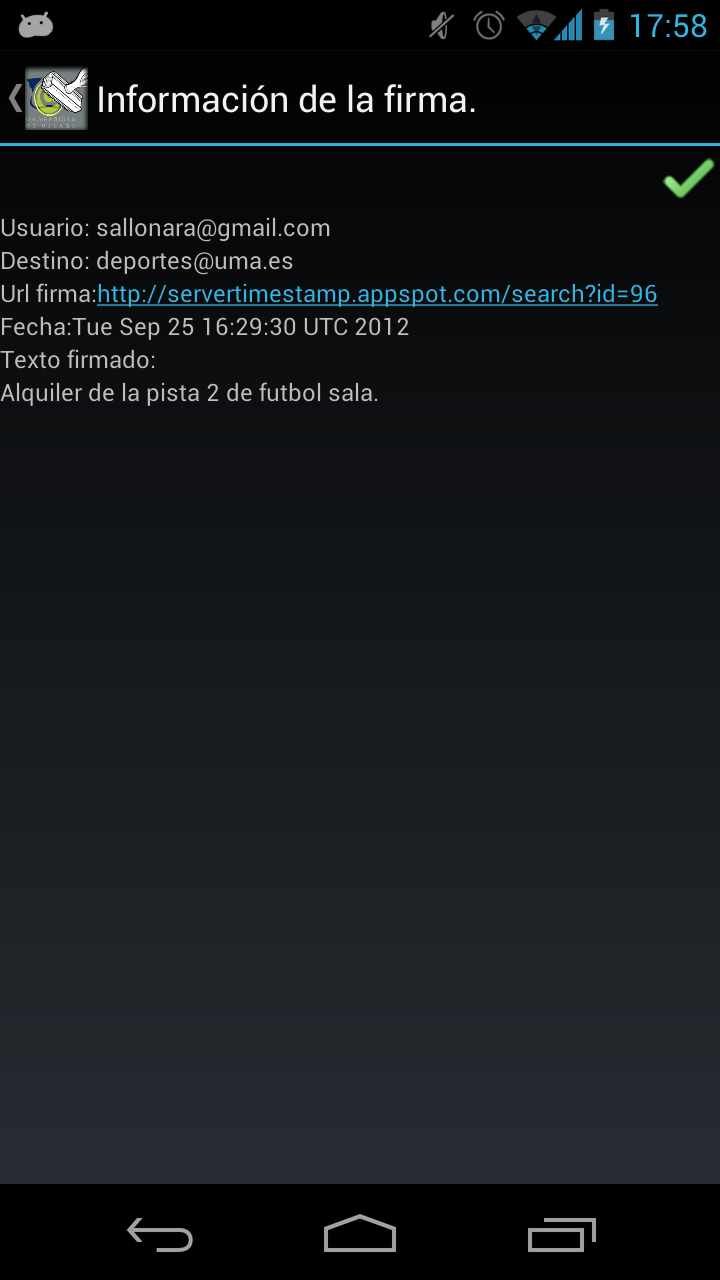
\includegraphics[scale=0.2]{./Android/imagenes/informacionFirma.png}
  \caption{Información de una firma realizada.}
  \label{fig:informacionFirma}
\end{figure}

\subsection{Detalles de la implementación.}

En la figura~\ref{fig:proyectoAndroid} podemos ver el proyecto de eclipse con todas las clases que hemos tenido que desarrollar, desde la conexión a la base de datos, el inicio de la aplicación, el cifrado, etc. La estructura del proyecto es la misma que ya hemos explicado anteriormente.

\begin{figure}
  \centering
    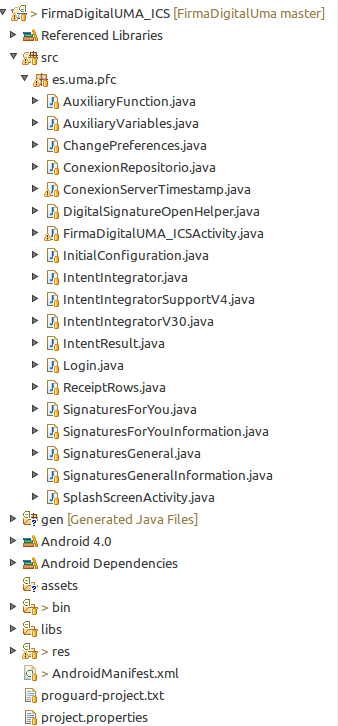
\includegraphics[scale=0.7]{./Android/imagenes/proyectoAndroid.png}
  \caption{Proyecto de Android en Eclipse.}
  \label{fig:proyectoAndroid}
\end{figure}

A continuación vamos a explicar cada una de las clases y la función que tiene dentro del proyecto.

\begin{itemize}

\item \textbf{AuxiliaryFunction.java:} en esta clase se han implementado todas las funciones que son usadas muchas veces en el proyecto, como puede ser la función que verifica si un certificado existe en un path determinado y si se puede abrir, también está la función que pasa de un array de bytes a una cadena de texto. 

\item \textbf{AuxiliaryVariables.java:} aquí se almacenan todas las variables comunes que vamos a necesitar para que la aplicación funcione correctamente. En el siguiente trozo de código podemos ver que son variables como el login con el cual se está logueado, la cookie para autentificación en el servicio, el key store con las claves para realizar las firmas, si la aplicación está sin internet para mostrar la base de datos que tengamos almacenados y no intentar bajar recibos nuevos y otras.

\begin{lstlisting}[style=Java]
private static Login LOGIN_GLOBAL;
private static Cookie COOKIE_GLOBAL;
private static KeyStore KEYSTORE_GLOBAL;
private static boolean WITHOUT_INTERNET;
private static List<ReceiptRows> LIST_RECEIPT;
private static String THEME;
\end{lstlisting}

Además de las variables tenemos todos los getter and setter de las variables.

\item \textbf{ChangePreferences.java:} esta clase es la encargada de realizar todo el manejo del cambio de preferencias si se produce. En la aplicación hemos usado una clase que proporciona Android para el almacenado de configuración llamada SharedPreferences, al usar este método Android proporciona listener para que cuando cambien se activen, de esta forma podemos controlar todos los cambios que realicemos actualizando en el acto la interfaz y guardando los datos en el acto. Un trozo de la clase en el que se puede observar como se crea y se implementa un listener para cuando se produzca un cambio en la configuración podamos actualizar tanto las shared preferences como la interfaz.

\begin{lstlisting}[style=Java]
EditTextPreference textPath = (EditTextPreference) findPreference(getActivity().getResources().getString(R.string.key_cert_path));

// Para que cuando cambie el texto lo cambie también en el título...
textPath.setOnPreferenceChangeListener(new OnPreferenceChangeListener() {
	public boolean onPreferenceChange(Preference preference, Object newValue) {
		EditTextPreference textPath = (EditTextPreference) preference;
		String s = (String) newValue;

		String pass = settings.getString("certificate_password", "NotValue");
		if (!pass.equals("NotValue")) {
			boolean check = AuxiliaryFunction.checkCert(s, pass);

			if (check) {
				textPath.setSummary(s);
				textPath.setText(s);
				Editor editor = settings.edit();
				editor.putString("path_certificate", s);
				editor.commit();
				return true;
			} else {
				textPath.setSummary("No se ha podido cargar el certificado,\nla ruta no es correcta");
				return true;
			}
		} else {
			textPath.setSummary("Password no guardado");
			return true;
		}

	}

});
\end{lstlisting}

Creamos la variable EditTextPreference donde mostraremos el password del certificado que estamos usando para firmar el texto. A continuación implementamos el listener OnPreferenceChangeListener, el cual se activará cuando digamos de cambiar el password del certificado. Podemos observar que cuando introducimos un nuevo password hacemos una comprobación para ver si después del cambio podemos seguir usando dicho certificado, si no es posible informamos al usuario diciendole que no se ha guardado el password.

\item \textbf{ConexionRepositorio.java:} en esta clase se ha implementado todo lo referente a interactuar con la aplicación web repositorio general. En dicha clase se ha implementado el método para añadir un recibo nuevo, listar todos los recibos que hay guardados, etc. Todos los métodos son estáticos para no tener que crear instancias de esta clase, además se vio que teníamos que crear una nueva conexión cada vez que queríamos añadir un nuevo nuevo recibo, por lo que no tendría sentido crea instancias de la clase. A continuación podemos ver el método que añade un nuevo recibo.

\begin{lstlisting}[style=Java]
public static String addRow(String plainText, String tokenTime, Account account, String to) {
	/*
	 * Primero se le codifican los espacios porque si no la función
	 * URLEncoder.encode los cambia por '+' y si el documento tiene '+'
	 * luego los pone como si fueran espacios
	 */
	String textoSinEspacios = plainText.replace(" ", "%20");
	textoSinEspacios = URLEncoder.encode(textoSinEspacios);
	String token = tokenTime.split(";;")[1];
	String fecha = tokenTime.split(";;")[2];
	String url = cadServer + cadAdd + cadServerTimestampSearch + token + "&texto=" + textoSinEspacios + "&token=" + token + "&usuario=" + account.name
			+ "&destino=" + to + "&fecha="+ fecha;
	String response = "";
	try {
		URL u1 = new URL(url);

		// Si queremos usar el proxy inicializarlo de esta forma, donde
		// sa es: SocketAddress sa = new
		// InetSocketAddress("proxy.alu.uma.es", 3128);
		// HttpURLConnection c = (HttpURLConnection)
		// u.openConnection(new Proxy(Proxy.Type.HTTP, sa));

		Cookie cookie = AuxiliaryVariables.getCOOKIE_GLOBAL();
	
		HttpURLConnection con1 = (HttpURLConnection) u1.openConnection();

		con1.addRequestProperty("Cookie", cookie.getName() + "=" + cookie.getValue());
		con1.setRequestMethod("GET");
		con1.connect();

		DataInputStream is1 = new DataInputStream(con1.getInputStream());
		response = is1.readLine();

		con1.disconnect();

	} catch (MalformedURLException e) {
		response = "MalformedURL";
		e.printStackTrace();
	} catch (ProtocolException e) {
		response = "ProtocolException";
		e.printStackTrace();
	} catch (IOException e) {
		response = "IOException";
		e.printStackTrace();
	}
	return response;
}
\end{lstlisting}

La función necesita una serie de parámetros para poder ser invocada, estos parámetros son los datos que necesitamos almacenar, como pueden ser el texto en claro, el token de tiempo que ha devuelto la aplicación web de timestamp, la cuenta con la que se está usando la aplicación y el destino, el resto de valores o los añade la aplicación web o la aplicación del móvil. A continuación se realiza la conexión con el servidor y se recibe una cadena donde se indica si se ha realizado bien la operación.

\item \textbf{ConexionServerTimestamp.java:} al igual que la clase anterior en esta se ha realizado todo lo relacionado con la aplicación web del servidor timestamp. Solo tiene una función que es la de añadir al servidor que tiene un aspecto similar a la mostrada en el apartado anterior.

\item \textbf{DigitalSignatureOpenHelper.java:} esta clase es la encargada de la creación de la base de datos SQLite, cuando vamos a necesitar tener acceso a ella hay que generar un objeto de dicha clase y llamar al contructor, que devuelve un objeto con el que podremos insertar, buscar o borrar elementos de la base de datos. Al pensar en el diseño de la aplicación se creyó necesario el uso de la base de datos para almacenar todos los recibos que se han realizado hasta la fecha, la aplicación sabe cual es el último recibo que tiene almacenado y solo pide a la aplicación web que le de los recibos nuevos, de esta forma de ahorra en tiempo de inicio de la aplicación y además en la cantidad de datos móviles que usamos.

Esta clase tiene que heredar de SQLiteOpenHelper que es la clase genérica que proporciona Android para manejo de la base de datos SQLite que tiene. Hay que implementar el constructor y dos métodos más obligatoriamente \lstinline{public void onCreate(SQLiteDatabase db);} y \lstinline{public void onUpgrade(SQLiteDatabase db, int oldVersion, int newVersion);}, el primero es usado para crear la base de datos en la primera ejecución y el segundo para actualizar la base de datos cuando sea necesario.

La base de datos se crea que con la siguiente sentencia SQL, podemos verla en el siguiente listado.

\begin{lstlisting}[style=Java]
static final String KEY_SEQ_NUM = "NUM_SEC";
static final String KEY_SIGN_URL = "URL_FIRMA";
static final String KEY_PLAIN_TEXT = "TEXTO_CLARO";
static final String KEY_TIME_TOKEN = "TOKEN_TIEMPO";
static final String KEY_USER = "USUARIO";
static final String KEY_VERIFY = "VERIFICADO";
static final String KEY_DESTINY = "DESTINO";
static final String KEY_DATE = "FECHA";

private static final String DIGITALSIGNATURE_TABLE_CREATE = "CREATE TABLE " + DIGITALSIGNATURE_TABLE_NAME + " (" +
	BaseColumns._ID + " INTEGER PRIMARY KEY AUTOINCREMENT," +
	KEY_SEQ_NUM + " TEXT, " +
	KEY_SIGN_URL + " TEXT, " +
	KEY_PLAIN_TEXT + " TEXT, " +
	KEY_TIME_TOKEN + " TEXT, " +
	KEY_USER + " TEXT, " +
	KEY_VERIFY + " TEXT, " +
	KEY_DESTINY + " TEXT, " +
	KEY_DATE + " TEXT );";
\end{lstlisting}

\item \textbf{FirmaDigitalUMA\_ICSActivity.java:} esta es la clase principal del proyecto, en ella se crea la activity principal de la aplicación. Se puede ver en el código que no extiende a la clase \lstinline{Activity}, si no que lo hace de \lstinline{FragmentActivity}, esto es así porque como ya hemos explicado anteriormente se han usado fragment para el diseño de la aplicación y no solo activitys. Además de esto se ha añadido funcionalidad mediante el uso de \lstinline{ViewPager} y \lstinline{TabsAdapter}, el primero para el uso del scroll lateral y el segundo para tener las dos pestañas de los recibos que el usuario a firmado y de los que es recipiente. En el siguiente trozo de código podemos ver la creación de los dos elementos que hemos dicho antes, junto con la action bar.

\begin{lstlisting}[style=Java]
mViewPager = new ViewPager(this);
mViewPager.setId(R.id.pager);
setContentView(mViewPager);

final ActionBar bar = getActionBar();
bar.setTitle("Firma digital UMA");
bar.setNavigationMode(ActionBar.NAVIGATION_MODE_TABS);

mTabsAdapter = new TabsAdapter(this, mViewPager);
mTabsAdapter.addTab(bar.newTab().setText("Repositorio general"), SignaturesGeneral.class, null);
mTabsAdapter.addTab(bar.newTab().setText("Firmas para ti"), SignaturesForYou.class, null);
\end{lstlisting}

Además de la creación de los elementos anteriores esta clase también es la encargada de crear los menús, que en la versión 4.0 de Android tienden a desaparecer, debido a la desapareción del botón menú de los nuevos terminales, pero que en las nuevas versión se añade a la action bar. A continuación podemos ver como se crean y añaden los botones de añadir un nuevo recibo, el de configuración o el de salir de la aplicación.

\begin{lstlisting}[style=Java]
@Override
public boolean onCreateOptionsMenu(Menu menu) {
	MenuInflater inflater = getMenuInflater();
	inflater.inflate(R.menu.main, menu);
	return true;
}
@Override
public boolean onOptionsItemSelected(MenuItem item) {
	switch (item.getItemId()) {

	case R.id.menuitem_add:
		Log.d(AuxiliaryVariables.TAG_DEBUG, "Add");
		IntentIntegrator intentQR = new IntentIntegrator(this);
		intentQR.initiateScan();
		return true;

	case R.id.menuitem_quit:
		Log.d(AuxiliaryVariables.TAG_DEBUG, "Quit");
		finish();
		return true;
	case R.id.menuitem_about:
		Log.d(AuxiliaryVariables.TAG_DEBUG, "About");
		Toast.makeText(context, "about", Toast.LENGTH_SHORT).show();
		return true;
	case R.id.menuitem_settings:
		Log.d(AuxiliaryVariables.TAG_DEBUG, "Settings");
		Toast.makeText(context, "ajustes", Toast.LENGTH_SHORT).show();
		Intent prefsIntent = new Intent(getApplicationContext(),
		        ChangePreferences.class);
		startActivity(prefsIntent);
		return true;
	}
	return false;
}
\end{lstlisting}

Además de la creación de la activity y de los menús es la encargada de llamar a la función de subir un recibo a la aplicación web después de recibir por medio de un intent el resultado de la lectura del código QR, se puede observar en este trozo de código.

\begin{lstlisting}[style=Java]
public void onActivityResult(int requestCode, int resultCode, Intent intent) {
	IntentResult scanResult = IntentIntegrator.parseActivityResult(requestCode, resultCode, intent);
	String plaintext = "";
	if ((plaintext = scanResult.getContents()) != null) {
		progressDialog = new ProgressDialog(activity);
		progressDialog.setMessage("Subiendo el recibo...");
		progressDialog.show();

		ConexionRepositorio.addRow(handler, plaintext);
		
	}
}
\end{lstlisting} 

\item \textbf{InitialConfiguration.java:} esta clase es la activity que se encarga de realizar la configuración de la aplicación cuando es la primera ejecución en un teléfono, en ella se tiene que configurar el certificado y su password y la cuenta. Es la encargada de crear las shared preferences para que la aplicación funcione correctamente. %TODO: poner una imagen de esto y revisarlo porque era mu cutre...

\item \textbf{InitialConfiguration.java, IntentIntegratorSupportV4.java, IntentIntegratorV30.java, IntentResult.java:} estas clases son las encargadas de la lectura de los códigos QR. Están hechas por ZXing y se distribuyen bajo licencia Apache License, Version 2.0. Proporcionan mediante un intent la posibilidad de lectura de códigos QR con su aplicación Barcode Scanner (figura~\ref{fig:barcodeScanner}) gratuita en Google Play, si no se tiene la aplicación instalada proporciona los métodos para hacerlo.
\end{itemize}

\begin{figure}
  \centering
    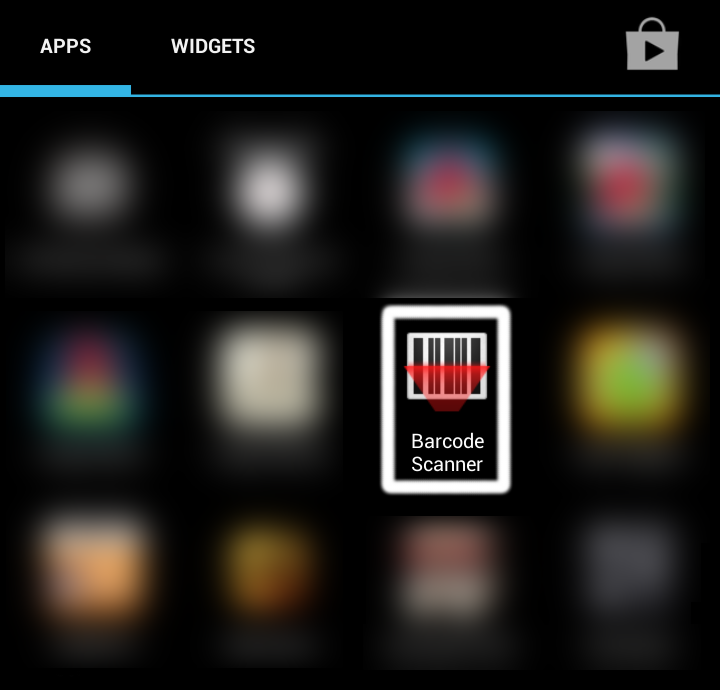
\includegraphics[scale=0.3]{./Android/imagenes/barcodeScanner.png}
  \caption{Aplicación Barcode Scanner.}
  \label{fig:barcodeScanner}
\end{figure}

\begin{itemize}
\item \textbf{Login.java:} esta clase es la encargada de realizar el login en la aplicación web Repositorio General. Google proporciona un método de login si se tienen las credenciales, cosa que tenemos gracias a que en Android se necesita tener una cuenta de Google para poder usar Google Play y los diferentes servicios que ofrece. La dirección a la que tenemos que dirigirnos es a: \url{https://repositoriorecibos.appspot.com/\_ah/login}. Esta clase tiene una variable privada que es el token de autentificación que conseguimos mediante la realización del login, para conseguirlo mostramos todas las cuentas de Google que hay configuradas en el terminal Android, cuando el usuario selecciona una de ellas iniciamos la conexión con el servidor y recibimos el token. Esto se hace todo el segundo plano para que la aplicación no se quede parada mientras se va a la página web y se consigue el token. En el código que sigue podemos ver el proceso de obtención del token.

\begin{lstlisting}[style=Java]
Thread t = new Thread() {
	public void run() {
		try {
			AccountManagerFuture<Bundle> future = manager.getAuthToken(account, "ah", null, activity, null, null);
			Bundle bundle;
			bundle = future.getResult();
			token = bundle.getString(AccountManager.KEY_AUTHTOKEN);
		} catch (OperationCanceledException e) {
			e1.printStackTrace();
		} catch (AuthenticatorException e) {
			e1.printStackTrace();
		} catch (IOException e) {
			e1.printStackTrace();
		}
	}
}.start();
\end{lstlisting} 

La parte mas interesante del código es en la llamada \lstinline{manager.getAuthToken(account, "ah", null, activity, null, null);} con esta función conseguimos la cookie donde está el token de acceso para posteriormente con la función \lstinline{bundle.getString(AccountManager.KEY_AUTHTOKEN);} conseguirlo.

La función \lstinline{public Cookie getAuthCookie(String authToken);} se puede ver en el siguiente trozo de código.

\begin{lstlisting}[style=Java]
public Cookie getAuthCookie(String authToken) throws ClientProtocolException, IOException {
	DefaultHttpClient httpClient = new DefaultHttpClient();
	Cookie retObj = null;
	String cookieUrl = gaeAppLoginUrl + "?continue=" + URLEncoder.encode(gaeAppBaseUrl, "UTF-8") + "&auth=" + URLEncoder.encode(authToken, "UTF-8");
	
	HttpGet httpget = new HttpGet(cookieUrl);
	HttpResponse response = httpClient.execute(httpget);
	if (response.getStatusLine().getStatusCode() == HttpURLConnection.HTTP_OK
			|| response.getStatusLine().getStatusCode() == HttpURLConnection.HTTP_NO_CONTENT) {

		if (httpClient.getCookieStore().getCookies().size() > 0) {
			retObj = httpClient.getCookieStore().getCookies().get(0);
		}

	}

	return retObj;
}
\end{lstlisting} 

En ella podemos ver que hacemos una conexión a la dirección \url{http://repositoriorecibos.appspot.com/\_ah/login?continue=http://repositoriorecibos.appspot.com&auth=token}, en la que se le indica el token de acceso y la url a la que tenemos que seguir cuando se realice el login. Una vez realizada la identificación devolvemos la cookie donde irá el token de acceso.

\item \textbf{ReceiptRows.java:} esta clase es la que representa un recibo, con ella se pueden crear objetos para almacenar todos los valores que necesitamos para tener un recibo identificado, como pueden ser el texto, la url de la firma, la fecha, el destino, etc. Este es el tipo de objeto que se usa para recoger la información de la base de datos y para almacenarla. Durante toda la ejecución de la aplicación tedremos una lista de objetos de esta clase para tener acceso a los recibos. Es una clase simple con un contructor con todos los valores que se guardan como parámetros y todos los getter y setter de las diferentes variables. También tiene definidas todas las constantes para el nombre de la tabla de la base de datos.

\item \textbf{SignaturesGeneral.java:} esta clase extiende a \lstinline{ListFragment}, es la lista de los recibos que el usuario a firmado. Es una de las dos pantallas principales de la aplicación, se puede ver en la figura~\ref{fig:signaturesGeneral}. Cuando se genera la interfaz se hace una consulta a la base de datos y se recibe un objeto de la clase \lstinline{Cursor}, en el cual se puede iterar para conseguir todos los recibos que has firmado. En el siguiente trozo de código podemos ver como se hace.
\begin{lstlisting}[style=Java]
DigitalSignatureOpenHelper digitalSignatureOpenHelper = new DigitalSignatureOpenHelper(activity);
	SQLiteDatabase sqLiteDatabase = digitalSignatureOpenHelper.getReadableDatabase();
	Cursor cursor = sqLiteDatabase.query(DigitalSignatureOpenHelper.DIGITALSIGNATURE_TABLE_NAME,
			new String[] { DigitalSignatureOpenHelper.KEY_PLAIN_TEXT }, null, null, null, null, null);
\end{lstlisting} 

\end{itemize}

\begin{figure}
  \centering
    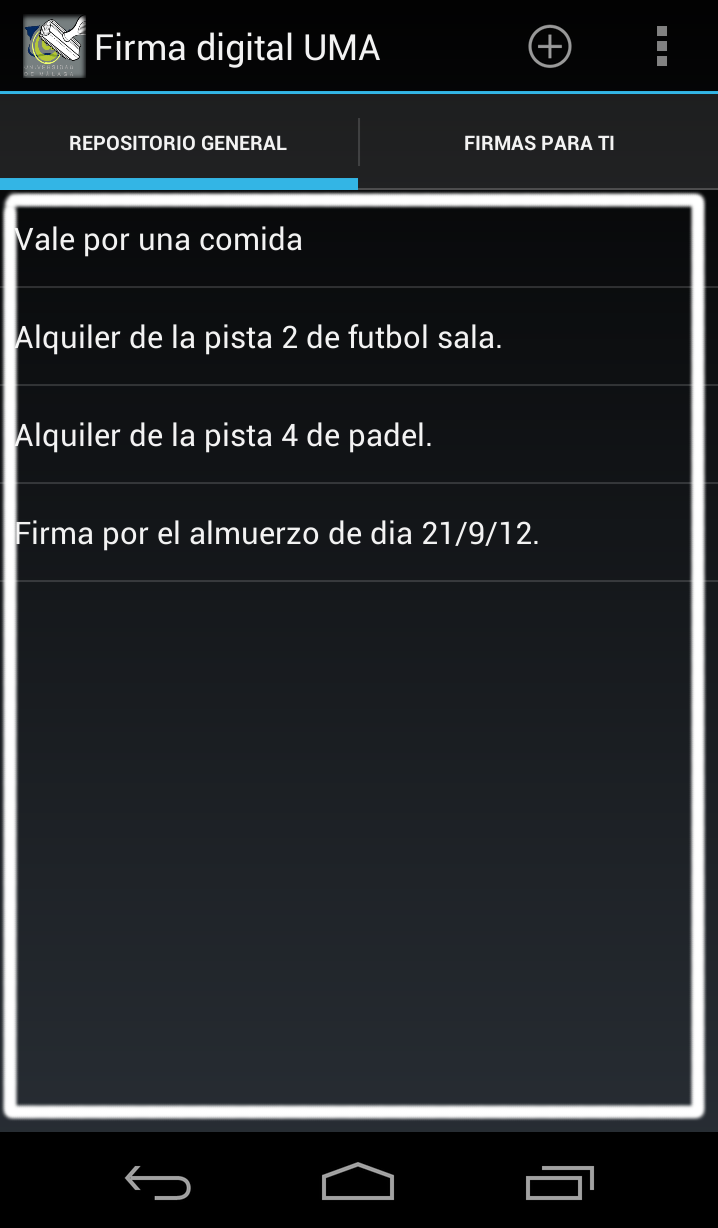
\includegraphics[scale=0.3]{./Android/imagenes/signaturesGeneral.png}
  \caption{Detalle fragment generado por la clase SignaturesGeneral.java.}
  \label{fig:signaturesGeneral}
\end{figure}

\begin{itemize}

\item \textbf{SignaturesGeneralInformation.java:} esta clase es la encargada de mostrar la información cuando pulsamos en algún recibo que hemos firmado. Es una clase que extiende de la clase \lstinline{Activity} y es la encargada de cargar la interfaz modelada en el XML \lstinline{signaturesgeneralinfo.xml} y mostrar toda la información del recibo que ha sido pulsado de la lista de recibos. Cuando se pulsa un recibo en la pantalla anterior que es la generada por \lstinline{SignaturesGeneral.java}, antes de cargar esta se le manda la posición que ha sido pulsada para después poder localizarla y acto seguido se muestra la información, esto se hace por medio de un \lstinline{Intent} al cual se le añade un valor entero con la posición. En el siguiente trozo de código podemos ver se recupera el valor, se realiza la consulta en la base de datos y se rellenan todos los campos donde mostraremos la información del recibo seleccionado.

\begin{lstlisting}[style=Java]
super.onCreate(savedInstanceState);
setContentView(R.layout.signaturesgeneralinfo);

Intent intent = this.getIntent();
int pos = intent.getExtras().getInt("position");

DigitalSignatureOpenHelper digitalSignatureOpenHelper = new DigitalSignatureOpenHelper(this);
SQLiteDatabase sqLiteDatabase = digitalSignatureOpenHelper.getReadableDatabase();
Cursor cursor = sqLiteDatabase.query(DigitalSignatureOpenHelper.DIGITALSIGNATURE_TABLE_NAME, new String[] { DigitalSignatureOpenHelper.KEY_USER,
		DigitalSignatureOpenHelper.KEY_DESTINY, DigitalSignatureOpenHelper.KEY_SIGN_URL, DigitalSignatureOpenHelper.KEY_PLAIN_TEXT,
		DigitalSignatureOpenHelper.KEY_VERIFY, DigitalSignatureOpenHelper.KEY_DATE }, null, null, null, null, null);

if (cursor.moveToPosition(pos)) {
	
	final ActionBar bar = getActionBar();
	bar.setTitle("Información de la firma.");
	bar.setDisplayHomeAsUpEnabled(true);

	TextView textUser = (TextView) findViewById(R.id.text_sign_general_user);
	TextView textDestiny = (TextView) findViewById(R.id.text_sign_general_to);
	TextView textUrl = (TextView) findViewById(R.id.text_sign_general_url);
	TextView textPlainText = (TextView) findViewById(R.id.text_sign_general_plain_text);
	ImageView imageVerify = (ImageView) findViewById(R.id.image_sign_general_verify);
	TextView textDate = (TextView) findViewById(R.id.text_sign_general_date);
	
	textUser.setText(textUser.getText() + " " + cursor.getString(0));
	textDestiny.setText(textDestiny.getText() + " " + cursor.getString(1));
	textUrl.setText(cursor.getString(2));
	textPlainText.setText(cursor.getString(3));

	String verify = cursor.getString(4);
	if (verify.equals("true")) {
		imageVerify.setImageResource(R.drawable.ok);
	} else {
		imageVerify.setImageResource(R.drawable.cancel);
	}
	textDate.setText(cursor.getString(5));

	sqLiteDatabase.close();
}
\end{lstlisting} 

Podemos ver como se genera el objeto \lstinline{DigitalSignatureOpenHelper} y se realiza la consulta con el método \lstinline{public Cursor query (String table, String[] columns, String selection, String[] selectionArgs, String groupBy, String having, String orderBy);}, a continuación generamos todos los \lstinline{TextView} necesarios para mostrar la información y los rellenamos con los datos.

\item \textbf{SignaturesForYou.java:} igual que su clase equivalente \lstinline{Signatures General.java} es la encargada de mostrar una lista con todos los recibos de los que se es destinatario, la estructura es practicamente idéntica, con solo una diferencia y es que se realiza un filtrado para que el campo destino sea el mismo que la cuenta de usuario usada en la aplicación. Podemos ver el resultado en la figura~\ref{fig:signaturesForYou}.

\end{itemize}

\begin{figure}
  \centering
    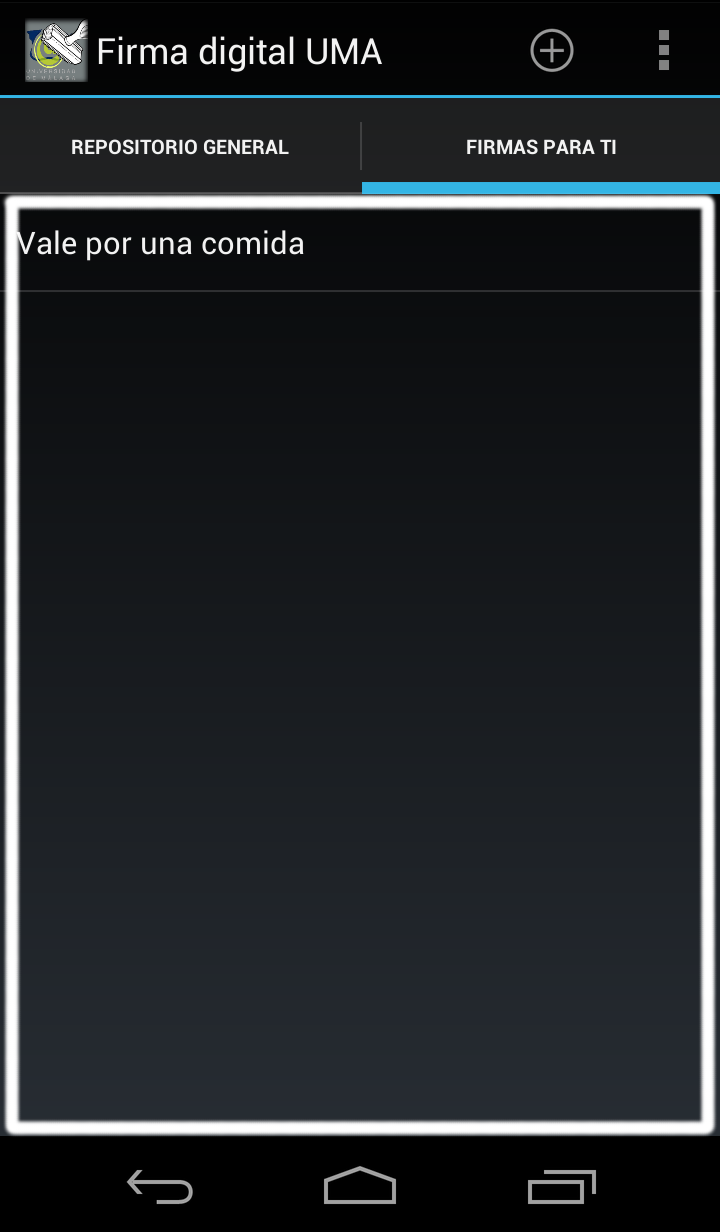
\includegraphics[scale=0.3]{./Android/imagenes/signaturesForYou.png}
  \caption{Detalle fragment generado por la clase SignaturesForYou.java.}
  \label{fig:signaturesForYou}
\end{figure}

\begin{itemize}

\item \textbf{SignaturesForYouInformation.java:} al igual que la clase \lstinline{SignaturesGeneralInformation.java} es la encargada de mostrar la información de los recibos que van dirigidos a tí. El proceso es igual que en \lstinline{SignaturesGeneralInformation.java}, se envia la posición que ha sido marcada y se busca dicho recibo y se muestra toda la información.

\item \textbf{SplashScreenActivity.java:} esta clase es la encargada de generar la primera activity que se muestra en la aplicación cuando se inicia, además de cargar todas las variables que serán usadas durante la ejecución. Esta clase crea una interfaz en la que solo muestra el logo de la aplicación y una barra progreso que muestra el proceso de carga, pero en backgroud comprueba que no sea la primera ejecución, si lo es llama a la clase \lstinline{InitialConfiguration.java} para generar la configuración, si no es la primera ejecución abre el archivo de preferencias compartidas y genera todos los objetos necesarios para la ejecución como pueden ser, la cuenta que utilizaremos posteriormente, el tema que estamos usando, hacemos el login en la aplicación web, el keystore que usaremos para firmar en la aplicación y a parte realizamos la conexión con la aplicación web Repositior General y conseguimos las filas que se hayan insertado nuevas añadiendolas a la base de datos de la aplicación para que posteriormente podamos usarlas sin tener que pedirlas al servidor, para ello se utiliza se tiene que parsear un objeto de tipo JSONArray, una vez realizadas todas esas acciones se procede a la inicialización de una nueva activity que genera la clase \lstinline{FirmaDigitalUMA_ICSActivity.java} y que dará lugar a la creación de la interfaz principal de la aplicación.

\end{itemize}



















